\documentclass[../ECON-281-Notes.tex]{subfiles}
\begin{document}
\chapter{Capturing Surplus}

In this chapter we will learn how the monopolist can achieve more surplus by \emph{using price discrimination} (charging consumer different prices for the same good) instead of using a uniform price for all consumer.

There are 3 different "degrees" of price discrimination
\begin{enumerate}
  \item \textbf{First Degree Price Discrimination} - The practice of attempting to price each unit at the consumer's maximum willingness to pay for that unit.
  \item \textbf{Second Degree Price Discrimination} - The practice of offering consumers a quantity discount.
  \item \textbf{Third Degree Price Discrimination} - Charging different uniform prices to different consumer groups. This type was covered in ECON 101 where monopolist charge a high price to consumers whose demand is less elastic and charge a low price to consumers whose demand is more elastic.
\end{enumerate}

\section{Condition for Price Discrimination}
There are certain conditions that must be satisfied for price discrimination to be able to generate more surplus to a firm.

\begin{enumerate}
  \item Firm must have some market power to price discriminate. This means the demand curve of the firm must be downward sloping. In case of perfect competition where the demand of the firm is horizontal the firm has no power to influence the price and hence cannot practice price discrimination.
  \item Firm must have some information about how much consumers are willing to pay and about their elasticities of demand.
  \item Firm must be able to prevent resale. The firm cannot prevent the resale of the product or service otherwise the consumer will buy from the low price market and resell the product in a high price market and take the profits for themselves.
\end{enumerate}

\newpage 

\section{First-degree Price Discrimination: Making the most from each consumer}

A profit maximizing monopolist who charges a uniform price will produce $Q_m$ and charge $P_m$ and achieves a producer surplus shown below.

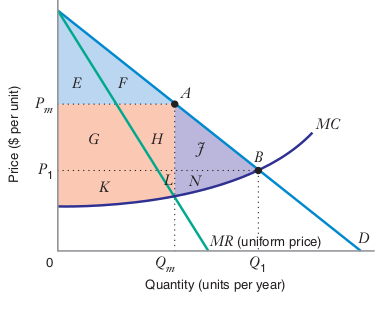
\includegraphics[width=\columnwidth]{assets/image_2021-11-30-11-32-46.png}

{\centering
\begin{DndTable}[color=PhbLightGreen]{XXX}
  ~ & \textbf{Uniform pricing} & \textbf{First-Degree Price Discrimination} \\
\textbf{Consumer Surplus} & $E+F$ & $0$ \\
\textbf{Producer Surplus} & $G+H+K+L$ & $E+F+G+H+J+K+L+N$ \\
\textbf{Total Surplus} & $E+F+G+H+K+L$ & $E+F+G+H+J+K+L+N$ \\
\textbf{DWL} & $J+N$ & $0$  \\
\end{DndTable}}

If there where uniform pricing there was a DWL but if the producer is charging the consumer the maximum price the consumer is willing to pay for each unit which is reflected by the market demand curve then the DWL is $0$. The producer will get all the surplus

\newpage

\section{Third Degree Price Discrimination: Different Prices for Different Market Segments}
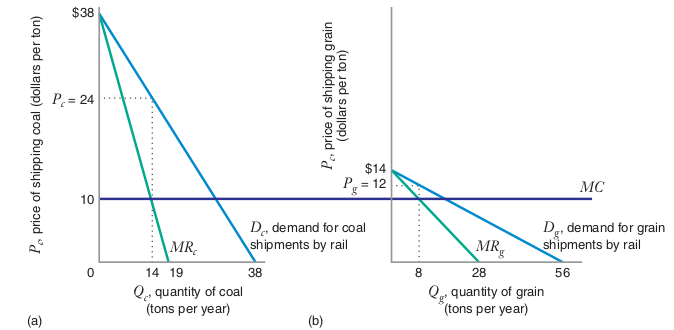
\includegraphics[width=\columnwidth]{assets/image_2021-11-30-11-43-03.png}
The first market (a) demand is steeper meaning less elastic than market b. Here the monopolist charges a higher uniform price in market a than in market b since consumers in market b are more sensitive to the price (more elastic).





\end{document}
